\section{PROCEDIMIENTO} 

\begin{itemize}
\subsection{Parte 1: Conectar a SQL Server desde Power BI Desktop }
	\item Para realizar los gráficos en PowerBi Desktop primero debemos conectarnos con nuestra base de datos, que ya tiene que tener la base de datos "AdventureWorks 2017".  \\Abrimos nuestro PowerBi desktop y procedemos a realizar la conexión a SQL server.
	\begin{figure}[h]
	\begin{center}
	\fbox{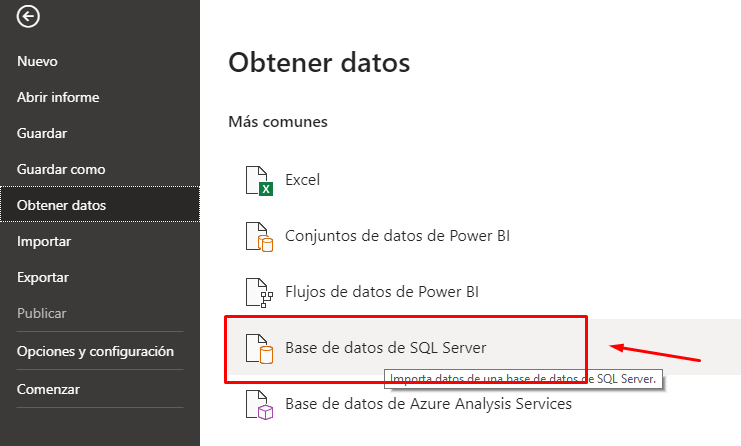
\includegraphics[width=12cm]{./Imagenes/tarea1}}
	\end{center}
	\end{figure}

\begin{figure}[h]
	\begin{center}
	\fbox{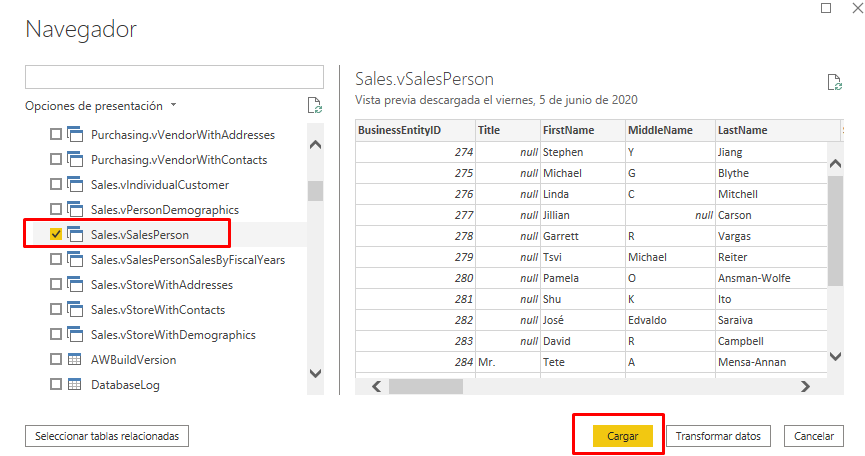
\includegraphics[width=13cm]{./Imagenes/tarea1_1}}
	\end{center}
	\end{figure}
\clearpage
	\begin{figure}[h]
	\begin{center}
	\fbox{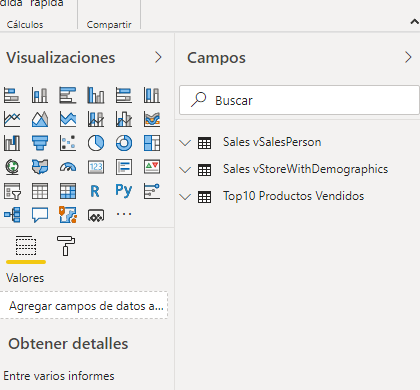
\includegraphics[width=11cm]{./Imagenes/tarea1_2}}
	\end{center}
	\end{figure}

	\item Una vez terminado de cargas los datos que necesitaremos, podremos visualizarlo en el panel lateral derecho de nombre "Campos".
	
     
\subsection{Parte 2: : Adicionar Gráficos al Reporte}
	\item En la parte 2 realizaremos los gráficos con la información de la base de datos que seleccionamos. Utilizaremos del panel de Visualizaciones los diferentes gráficos que nos ofrecen.

\begin{itemize}
	\item{\textbf{1. Cantidad de Ventas del personal: }} Gráfico de Columna Apilada que nos muestra el reporte de la cantidad de ventas de cada personal de ventas.
	\item {\textbf{2. Número de Empleados por especialidad: }}En el gráfico de Pie, muestra los la cantidad de empleados que tiene la empresa según su especialidad.
	\item {\textbf{3. Top 10 Productos vendidos: }}El gráfico de Donut, muestra el top 10 de los productos más vendidos. Podremos visualizarlo representados en los diferentes colores en el gráfico.
	\item {\textbf{4. Ventas Anuales y Beneficios Anuales: }}En el segundo gráfico de Columna Apilada podremos visualizar la cantidad de ventas anuales y los beneficios que ha traido. 
	\end{itemize}

\begin{figure}[h]
	\begin{center}
	\fbox{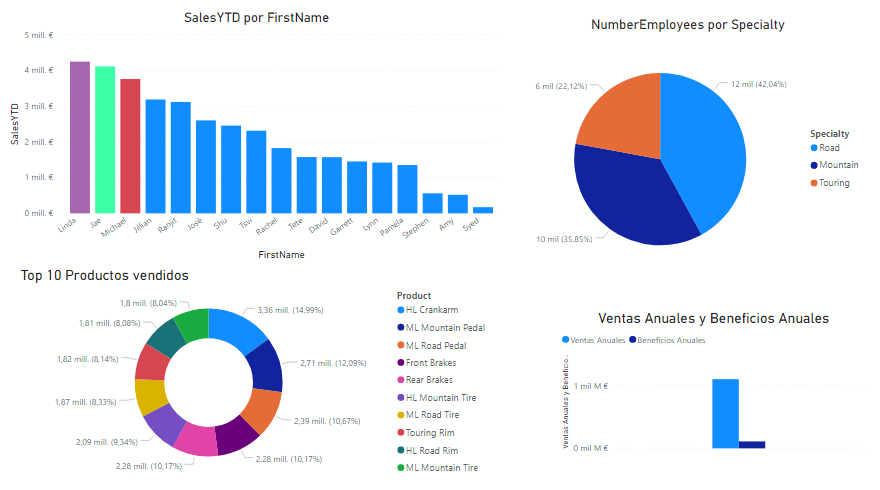
\includegraphics[width=15cm]{./Imagenes/tarea2}}
	\end{center}
	\end{figure}
		
\clearpage

\subsection{Parte 3: Publicar el reporte en el portal de Power BI}
	\item Cuando los gráficos esten listos, seleccionamos la opción de "Publicar" que nos ofrece PowerBi y poder subirlo a nuestra "Área de Trabajo". Cuando damos a "Aceptar" el archivo se irá subiendo a nuestra cuenta.

\begin{figure}[h]
	\begin{center}
	\fbox{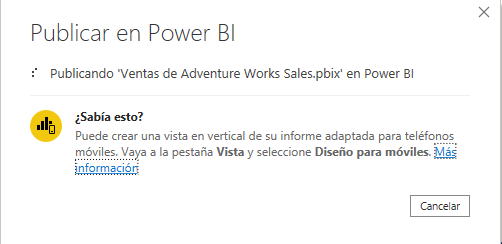
\includegraphics[width=11cm]{./Imagenes/tarea3}}
	\end{center}
	\end{figure}

\item Una vez se haya terminado de subir, abrimos nuestra cuenta desde la página web de Microsoft PowerBi y podremos visualizar nuestro trabajo ahí.

\begin{figure}[h]
	\begin{center}
	\fbox{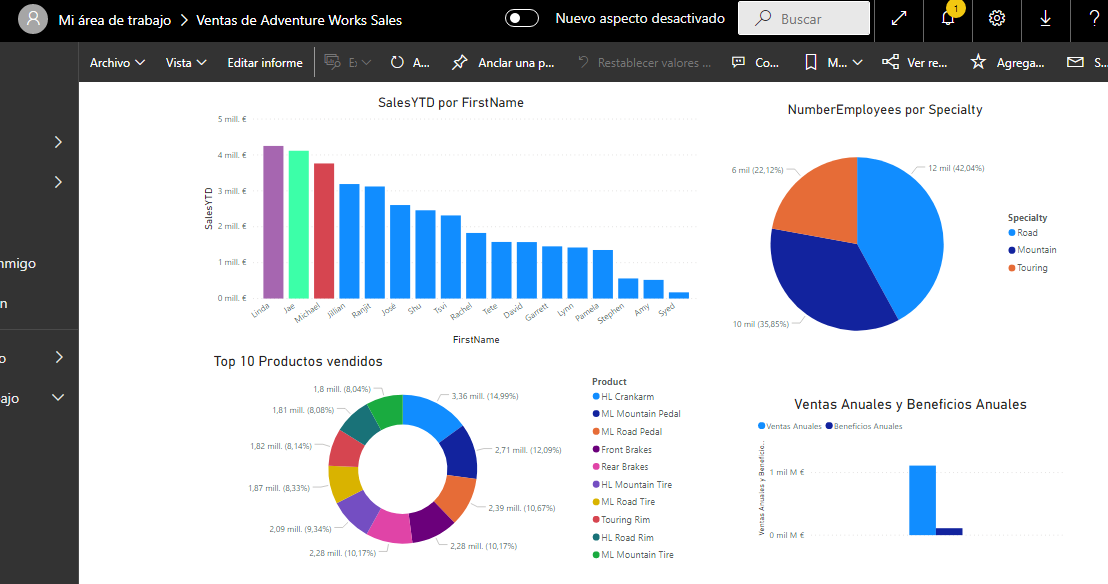
\includegraphics[width=14cm]{./Imagenes/tarea3_1}}
	\end{center}
	\end{figure}

\end{itemize}
		